\documentclass[12pt]{article}
\usepackage{graphicx}
\usepackage[a4paper,margin=1in]{geometry}
\usepackage{hyperref}
\usepackage{amsmath}
\usepackage{amssymb}
\usepackage{natbib} 
\title{Introduction}
\begin{document}
\maketitle
%\chapter*{Introduction}

Drug discovery is an arduous journey with many unknowns throughout the path that may lead to failures. To perform a large number of trials iteratively, computer simulations are convenient enabling tens of thousands of calculations. This sheer number of calculations can provide crucial insights, and possibly, rule out dead ends very early in the discovery cycle. Drug discovery is known to be a multi-faceted science that requires a great deal of art and innovative thinking, and often luck plays a good role. For the latter factor, we have no control, however, the best we can do is to base our science on solid foundation. In computational chemistry and biology, we often aske an important question- how do we train computers to think like humans? However, this is not a worry because we do not need to train computers to think like humans. As a matter of fact, computer are extremely fast but dumb machines. Whereas humans are extremely slow, lazy yet smart thinkers. Now, the division of labour between humans and computers should be straightforward; let the computers do the repetitive tasks of solving several complex mathematical equations that can be programmed to describe chemistry and biology. This is done by employing the laws of physics that govern the movement of the atoms, and therefore molecules. Humans can focus on the complex decision-making steps that are beyond mathematical equations. However, with generative artificial intelligence (\textbf{GenAI}), computers can perform some level of thinking. However, their chemical and biological validity, in a general sense, remains to be tested. GenAI, therefore, deserves an appreciation to at least recognise the idea that computers could be made to think, not in a biological sense, rather in a mathematical sense, which can be converted to chemical or biological models. However, the latter part has been extremely challenging and yet to be conquered entirely. 

The aim of this book is to ensure that the reader, perhaps, a beginner is aware of many assumptions that enable quick calculations. Also, thoroughly understand the limitations of these methods and to use them to perform calculations that they are meant or developed for. There are certain critical assumptions that ensure the speed of the calculations are, neglecting the solvation effect, and neglecting the entropy part of the free energy of binding. These, and more limitations will discussed in great detail in this later chapters of this book. It must be noted that such assumptions are somewhat important to ensure that the calculations are fast enough to finish several hundreds or thousands docking calculations per day, as warranted to virtually screen huge databases that comprise few million to billion molecules. 

This chapter can be treated as a short summary on topics that will be covered in great detail in the following chapters. Note that this book is intended to be a practical guide, therefore, we will emphasise more the practical aspects of molecular docking one needs to know before employing it to generate lead ideas or hit finding. We have made efforts to cover the theoretical foundations on topics that we deem crucial to successfully apply molecular docking. Depsite effects, we do not claim this book to be comprehensive text to cover all theoretical foundations on molecular docking. We further encourage readers to start practicing molecular docking, even though one may think they know nothing on this topic. We claim, with some personal experience on learning several computationals tools, the most learning happenings by trying first, and then consulting books like this one to sharpen your understanding. 

\section{Molecular Recognition and Binding}
Understanding protein-ligand interactions at the atomic or molecular level is central to studying how small molecules interact with their biological receptor(s). Thus binding phenomenon may involve, but not limited to, multiple types of non-covalent interactions such as hydrogen bonds, electrostatic interactions, van der Waals forces, and hydrophobic interactions. The binding affinity between a ligand and its receptor can be determined by the sum of favourable and unfavourable interactions, with the overall binding affinity dictating the strength of the complex. Protein-ligand binding affinity prediction quantifies the binding strength, providing crucial insights for lead optimisation by changing functional groups that lead to maximum gains\cite{CH1_13}. 

The binding affinity is determined experimentally in the form of inhibition constants (K$_\text{i}$), dissociation constants (K$_\text{d}$), or half-maximal inhibitory concentrations (IC$_\text{50}$). If one is using isothermal calorimetry, then direct measurements to thermodynamic qualities like the change in enthalpy due to ligand binding ({$\Delta$}H), and the change in entropy (T{$\Delta$}S) can be made. However, experimental methods are expensive and time-consuming, thus, efficient computational methods are capable of making accurate protein-ligand binding affinity predictions are time and cost saving methods. Such accurate and high-quality computational methods can reduce the number expensive experiments by filtering unwanted molecules. The downside of computational methods are that they are heavily dependent on the empirical parameters used to make computing tractable.

\section{Historical Background}

\subsection{Early Foundations}
The conceptual foundations of structure-based drug design can be traced back to the early 20$^{\text{th}}$ century with Emil Fischer’s lock-and-key theory proposed in the late 1800s\cite{CH1_1}. This theory postulated that ligands fit into receptors like a key into a lock, representing the first mechanistic understanding of molecular recognition. This concept was later refined by Daniel Koshland’s induced-fit theory in 1958\cite{CH1_2}, which recognized that proteins are dynamic in nature that undergo conformational changes upon ligand binding. The induced-fit theory suggested that the binding site of the protein is continually reshaped by interactions with the ligands as they interact with the protein, providing a more accurate description of binding events than the rigid treatment.

\subsection{The Birth of the Protein Data Bank}
A pivotal moment in the history of SBDD came in 1971 with the establishment of the Protein Data Bank (PDB) as the first open-access, digital-data resource in biology\cite{CH1_3}. The PDB was created to gather structural biologists at a single platform and has evolved from being a collaboratory network to a full-fledged database with an extensive list of protein structures, nucleic acid-containing structures, and computational models. The availability of three-dimensional atomic level structures of biomacromolecules determined using X-ray crystallography, nuclear magnetic resonance (NMR) spectroscopy, and electron microscopy fundamentally transformed drug discovery.

\subsection{Structural biology Revolution}
Structural biology has undergone tremendous improvements over the past few decades that led to a direct impact on structure-based drug design (SBDD)\cite{CH1_4}.  X‑ray crystallography provided the first atomic‑resolution views of protein–ligand complexes and established the modern SBDD. High‑resolution crystal structures give crucial information on binding pockets, hydrogen‑bond networks, and water-mediated contacts. This information improves our understanding about the drug-receptor interactions with atomic details. Over time, improvements in crystallization methods, synchrotron sources, and detectors increased throughput and resolution, making co‑crystal structures a routine decision‑making tool in medicinal chemistry. Furthermore,  NMR spectroscopy extended this static picture representation of proteins by resolving their stucture in solution under near‑physiological conditions\cite{CH1_4}.  
Most recent advancement has been in the field cryogenic electron microscopy (Cryo-EM). Improvements in direct electron detectors, image processing algorithms, and microscope stability has enabled near atomic level resolution for large complexes and membrane proteins that were previously intractable to crystallography or NMR. Single particle cryo‑EM routinely yields structures of GPCR–G protein complexes, ion channels, transporters, and multi‑subunit assemblies in multiple functional states, providing unprecedented insights into conformational landscapes and ligand‑induced transitions. This has transformed SBDD for membrane proteins: structures of clinically important targets such as TRP channels, CFTR, and GABA receptors have revealed binding sites, gating mechanisms, and off‑target liability determinants that now guide design of safer and more selective small molecules\cite{CH1_5}.

\subsection{Evolution of molecular docking methods}
Molecular docking has evolved from a geometric fitting algorithm on rigid receptor and ligands to algorithms that can handle flexibility in ligand and receptor simultaneously. The first widely recognized docking approach was developed by Kuntz and co‑workers in 1982, implemented in the program DOCK.\cite{CH1_6} This method treated both receptor and ligand as rigid bodies, and emphasized geometric complementarity: ligands were positioned in binding sites by matching molecular shape using spheres and surface representations. This “first generation method” established the conceptual framework of pose prediction and ranking, however neglected conformational flexibility and detailed energetics due to computational limitations.
In the 1990s and early 2000s, many groups followed with major improvements to increase the accuracy of the docking method. Search algorithms such as systematic search, Monte Carlo based search, and genetic algorithms were employed to enhance the ligand sampling to find the bioactivity conformation. Since accuracy of the docking methods also depends on the scoring functions, empirical and force field‑based scoring functions were developed to approximate binding affinity.\cite{CH1_7, CH1_8} Programs such as AutoDock incorporated a Lamarckian genetic algorithm and grid‑based energy evaluation, that allowed a routine docking of ligands with many rotatable bonds against rigid receptors.\cite{CH1_9} As the speed to docking ligands increased, this allowed for docking-based virtual screening of large chemical databases for hit identification, which significantly improved the productivity of early phase drug discovery. 

The next logical improvement focused on adding receptor flexibility to account for induced-fit effect to mimic physiogical binding phenonmenon. However, the additional degree of freedom came a the cost of computational speed\cite{CH1_8}. This was partially remedied by ensemble docking, which means instead of docking with receptor flexibility, docking was carried out on several conformations of the proteins that might have reported experimentally or with short runs of moecular dynamics simulations. 
Another milestone in the development of molecular docking methods was the ability to address covalent docking. Several of the drugs in the oncology section show their anticancer properties by covalently binding to its target. This was possible with algorithms capable of sampling non-covalent pre-reactive ligand topologies, followed by refining poses using post-reactive topologies that include the covalent bond\cite{CH1_11,CH1_12}.

Recent developments focused on leveraging the machine learning–based scoring functions, explicit treatment of structural water, and dynamic docking approaches that couple molecular dynamics with docking searches\cite{CH1_10}. Taken together, these improvements over several decades have significantly improved both computational speed and accuracy. Now a days, screening a large libray of millions to billion molecules is tractable. This can be equally attributed to parallel improvements in docking algorithms and computing power of modern day computers or supercomputers.

%START EDITING HERE
\section{Structure-based drug design}
Structure-based drug design (SBDD) uses the knowledge of the receptor structure and the binding site thereof to understand the shape of ligands and the type of interactions required for binding. it involves the use of three-dimensional structures of biological macromolecules, such as proteins or nucleic acids, to guide the design of molecules that can bind to the target protein and modulate its activity. The lock-and-key hypothesis is the main assumption for developing software tools. Therefore, the quality of the results depend on two things assuming the software used is accurate (more on this in later chapters explaining why this is not always true):
\begin{itemize}
    \item Quality of the receptor structure
    \item Confidence with which the binding site information is known
\end{itemize}
The objective of molecular docking is to enables us to predict the binding modes, and thus, affinities of small molecules to their target receptor. It models the interaction between the atoms of small molecule and receptor. Generally speaking, molecular docking is possible between any two (or more) chemical or biological entities, such as protein-protein, protein-DNA, protein-RNA and all such combinations that are biologically observed. All aforementioned binding and recognition follows the same rules of interactions governed by laws of physics. However, computationally, different potential energy functions are needed to model these binding with accuracy. We  mainly focus on small molecule protein docking, nevertheless, these discussion should be applicable to other kind of docking. 

\subsection{Fundamental Principles of Structure-Based Drug Design}
\subsubsection{The SBDD Paradigm}
Structure-based drug design is fundamentally dependent on knowledge of the three-dimensional structure of the biological target. The iterative process of SBDD begins with the selection of a potential target, followed by ligand identification. The target may be a macromolecular protein or enzyme involved in biosynthetic pathways. After selection of the target, extraction, purification, and determination of the structure of the protein are crucial processes.
The 3D structure of the protein is developed using sophisticated techniques including X-ray crystallography, nuclear magnetic resonance spectroscopy, and cryo-electron microscopy. Once the structure of the target is identified, it is necessary to investigate the electrostatic properties of the binding site such as presence of cavities, clefts, amino acid sequences, and allosteric pockets. Using various available computer algorithms, drug-like molecules from large databases of small molecules or fragments of compounds can be docked into the binding cavities of the target protein.

\subsection{The SBDD Workflow}
Figure \ref{fig:sbdd_workflow} shows a typical workflow for computational drug discovery. Depending on the chemical and biological information available, one might proceed by the structure-based approach or ligand-based. 
\begin{figure}[hbt!]
    \centering
    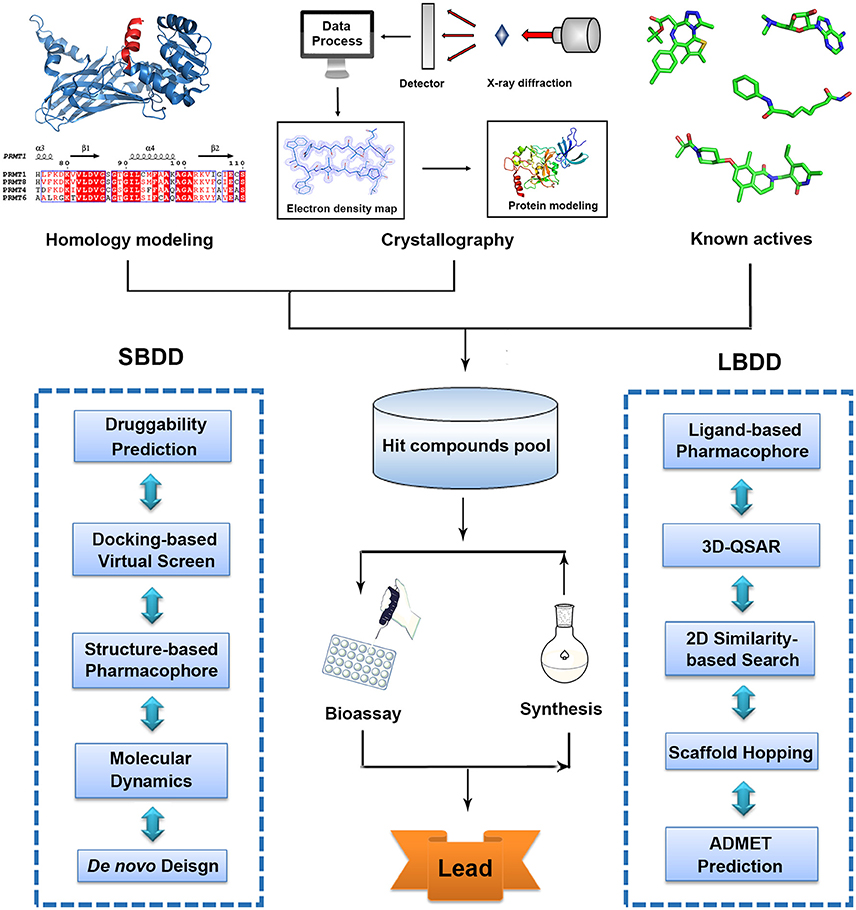
\includegraphics[width=1\textwidth]{../Figs/SBDD.jpg}
    \caption{A typical computational workflow for drug design. This figure also compares an alternative workflow called ligand-based drug design (LBDD), which is used when receptor information is not available. This image is reproduced from  10.3389/fchem.2018.00057 under the Creative Commons Attribution License (CC BY) licence.} 
    \label{fig:sbdd_workflow}
\end{figure}

\subsubsection{Druggability and Target Selection}
Druggability refers to the likelihood that a biological target can be modulated by a small molecule or biological drug. The first step in SBDD is the choice of an appropriate target, followed by evaluation of the structure of that target. Targets must possess characteristics that make them amenable to small molecule binding, including accessible binding sites with suitable geometry and chemical properties. Artificial intelligence models, particularly supervised machine learning algorithms, can now be trained on datasets to differentiate known druggable and non-druggable targets based on structural properties of the protein, its function, interaction partners, and its role in disease pathways.
\subsubsection{Determination and Preparation}
The SBDD workflow begins with obtaining the three-dimensional structure of the target protein. Structures can be obtained from the Protein Data Bank, which currently holds over 155,000 atomic-level 3D structures of biomolecules. When experimental structures are not available, protein modeling including homology modeling and ab initio techniques allows for creation of three-dimensional protein structures.
Selection of appropriate protein structure from the PDB is a critical step, as multiple crystal structures are often available for the same protein. A systematic approach for selecting the right type of protein structure must consider factors such as resolution, completeness, presence of ligands, and biologically relevant conformations. Recent advances include AlphaFold, which has revolutionized life sciences by predicting over 200 million protein structures available in the AlphaFold Database, far exceeding the number of experimentally resolved structures.

\subsubsection{Ligand Library Preparation}
After target structure preparation, the next step involves preparing libraries of compounds for virtual screening. Ligand preparation includes generating three-dimensional coordinates, assigning proper protonation states, and optimizing geometries. Compound libraries can range from commercially available compounds to virtual libraries representing chemical space that could be synthesized.

\subsubsection{Virtual Screening}
Virtual screening is a computational technique used to search large libraries of compounds and identify those most likely to bind to a drug target. Structure-based virtual screening uses molecular docking to test large libraries of compounds for potential binding to target proteins. Computer-aided drug design allows many molecules to be analyzed in a short time and enables simulation and prediction of several essential factors.
The virtual screening process typically involves multiple stages of filtering and refinement. Initial rapid screening of large compound collections using fast scoring methods is followed by more detailed analysis of top-ranked compounds using more sophisticated scoring approaches. Consensus virtual screening between multiple docking programs can increase reliability of results.
Hit Validation and Optimization
Top-scoring molecules from virtual screening with high affinity toward target protein are synthesized and tested in in vitro biochemical assays. Ligands with desired therapeutic activities are further evaluated for efficacy, affinity, and potency studies. Structural insights into the complex of ligand-protein assist the analysis of variety of binding conformations and interactions.
The availability of 3D structure of the target protein in complex with promising ligands offers detailed evidence of intermolecular features aiding in molecular identification process and binding pattern of the ligand. This iterative process of structure determination, docking, synthesis, and testing continues until optimized lead compounds are identified.







%\subsection{Molecular Docking: Concepts and Methods}
%Fundamentals of Molecular Docking
%Molecular docking is a computational technique that predicts the binding affinity of ligands to receptor proteins. The docking process involves two basic steps: prediction of the ligand conformation as well as its position and orientation within binding sites (usually referred to as pose) and assessment of the binding affinity. These two steps are related to sampling methods and scoring schemes, respectively. Docking has become a key tool in drug discovery and molecular modeling applications, with its reliability depending on the accuracy of the adopted scoring function.
%The scoring function guides and determines the ligand poses when thousands of possible poses are generated. It can be used to determine the binding mode and site of a ligand, predict binding affinity, and identify potential drug leads for a given protein target. Despite intensive research over the years, accurate and rapid prediction of protein-ligand interactions remains a challenge in molecular docking.
%Binding Site Identification
%Knowing the location of the binding site before docking processes significantly increases docking efficiency. In many cases, the binding site is known before docking ligands into it, and information about the sites can be obtained by comparison of the target protein with a family of proteins sharing similar function or with proteins co-crystallized with other ligands. In the absence of knowledge about the binding sites, cavity detection programs or online servers such as GRID, POCKET, SurfNet, PASS, and MMC can be utilized to identify putative active sites within proteins. Docking without any assumption about the binding site is called blind docking.

%Rigid vs. Flexible Docking
%The treatment of molecular flexibility represents a fundamental consideration in docking methodology. Early docking methods treated both ligand and receptor as rigid bodies based on the lock-and-key theory. Docking has been performed with a flexible ligand and a rigid receptor for a long time and remains the most popular method in use. This approach balances computational efficiency with reasonable accuracy for many applications.
%Considering the limitation of computer resources, flexible ligand docking with rigid receptors dominated the field, though recently many efforts have been made to deal with the flexibility of the receptor. Flexible receptor docking, especially backbone flexibility in receptors, still presents a major challenge for available docking methods. The induced-fit theory suggests that ligand and receptor should be treated as flexible during docking, as this could describe binding events more accurately than rigid treatment.
%Docking Algorithms
%Multiple algorithmic approaches have been developed for conformational sampling in molecular docking. Common search algorithms include genetic algorithms, Monte Carlo methods, simulated annealing, and systematic search approaches. The Lamarckian Genetic Algorithm implemented in AutoDock4 successfully modeled flexible ligand binding, particularly useful in complex systems requiring in-depth torsional and conformational exploration.
%AutoDock Vina introduced a multithreaded architecture that outperformed AutoDock4 by up to 100 times in docking throughput. Using benchmark datasets, Vina correctly placed native-like poses in the top three results in more than 93\% of situations, particularly excelling in polar and charged receptor settings. The Attracting Cavities algorithm represents another important approach, positioning cloud points in protein cavities and using these as guides for ligand placement and optimization.

%Major Docking Software
%Several molecular docking programs have become widely adopted in the drug discovery community. AutoDock and AutoDock Vina are among the most popular open-source docking programs, with AutoDock Vina highly cited and widely used. AutoDock4 uses flexible ligand and protein side chain modeling with a Lamarckian Genetic Algorithm, predicting binding of small molecules to receptors of known 3D structure.
%GOLD (Genetic Optimization for Ligand Docking) is a docking program based on genetic algorithms with flexible ligand and partial protein flexibility. Glide offers standard precision, extra precision, and virtual high throughput screening models based on exhaustive search. DOCK performs flexible ligand docking using a rigid body docking approach with geometric matching algorithms. FlexX and FlexE provide incremental build-based docking with flexible ligands in FlexX and flexible protein and ligand in FlexE.
%More recent developments include SwissDock 2024, which offers molecular docking using the Attracting Cavities algorithm and AutoDock Vina, providing free web-based services for small-molecule docking. The latest version of Attracting Cavities (AC 2.0) allows for random modification of initial ligand orientation and box center to limit dependence on starting conditions, and includes capabilities for covalent ligand-protein docking.

%Scoring Functions
%Role and Importance
%Scoring functions are mathematical functions used to approximately predict the binding affinity between two molecules after they have been docked. They are among the most important components in structure-based drug design. During the docking process, the search algorithm investigates a vast amount of conformations for each molecule, and scoring functions evaluate the quality of these docking poses, guiding the search methods toward relevant ligand conformations.
%The scoring function calculates a score or binding affinity of a particular pose, representing the thermodynamics of interaction of the protein-ligand system, to distinguish true binding modes from all others explored and rank them accordingly. Scoring functions are typically employed to predict the binding conformation, binding affinity, and binary activity level of ligands against critical protein targets in disease pathways.

%Goals of Scoring Functions
%Scoring functions must accomplish three primary tasks. The first requirement is the ability to distinguish experimentally observed binding modes, associating them with the lowest binding energies of the energy landscape from all other poses found by the search algorithm (pose prediction). The second goal is to classify active and inactive compounds during virtual screening. The third is prediction of absolute binding affinity, ranking compounds correctly according to their potency (binding affinity prediction), which is the most challenging task, mainly in de novo design and lead optimization.
%An ideal scoring function would be able to perform all three tasks effectively. However, given several limitations of current scoring functions, they exhibit different accuracies on distinct tasks due to modeling assumptions and simplifications made during their development phase. Scoring functions are intrinsically associated with their main purpose, and docking protocols can adopt different scoring functions for each step.
%Types of Scoring Functions
%Four basic types of scoring functions have been developed: physics-based, empirical, knowledge-based, and machine learning-based scoring functions. Physics-based (force-field) scoring functions calculate binding affinity using molecular mechanics force fields and statistical thermodynamics approaches. These methods attempt to estimate the binding free energy by summing various energetic terms including van der Waals interactions, electrostatic interactions, and solvation effects.
%Empirical scoring functions use regression methods to fit coefficients of physically motivated functional terms to experimental binding affinity data. These functions typically decompose the binding free energy into individual components such as hydrogen bonding, hydrophobic interactions, and entropic penalties. Knowledge-based scoring functions derive their parameters from statistical analysis of protein-ligand complex structures in databases like the PDB. They are based on the inverse Boltzmann principle, converting observed frequencies of interatomic contacts into pseudo-energy potentials.
%Machine learning-based scoring functions represent the newest category, using artificial intelligence and neural networks to learn patterns from training data. These approaches have shown promise for outperforming traditional scoring functions while displaying greater generalizability and versatility. Deep learning models can capture complex nonlinear relationships between structural features and binding affinities.

%Scoring Function Performance and Evaluation
%The performance of scoring functions is generally evaluated regarding four aspects: docking power (ability to detect native binding mode from decoy poses), ranking power (ability to rank compounds by potency), screening power (ability to distinguish active from inactive compounds), and scoring power (ability to predict absolute binding affinities). The root-mean square deviation (RMSD) is the most commonly used metric to assess docking power performance.
%Standard benchmarks are of great importance for objective assessment of scoring functions, providing reproducible and reliable ways to compare different methods. PDBbind, DUD-E, and DEKOIS 2.0 are examples of widely used benchmarks for evaluating scoring functions. However, one major stumbling block to advancement of protein-ligand docking validation has been the lack of a standard test set agreed upon and used by the entire community.
%Most of today’s scoring functions are generic models derived from large-scale experimental data of ligand-target complexes and are presumably applicable to all sorts of target classes. However, previous comparative studies have revealed that a universally accurate scoring function is still out of reach. Chemical properties and molecular spaces significantly influence the performance of scoring functions. Effective training of scoring functions requires careful attention to quality of training data and methodologies, with emphasis on the need for robust training strategies to produce consistent and generalizable scoring functions.

%Consensus Scoring
%Consensus scoring techniques have emerged as a strategy to improve docking reliability by combining predictions from multiple scoring functions. The rationale behind consensus scoring is that different scoring functions have different strengths and weaknesses, and combining them can compensate for individual limitations. Consensus virtual screening approaches between different docking programs, such as AutoDock Vina and DOCK 6, have demonstrated the ability to achieve satisfactory results and increase the reliability of docking.


\section{Current Challenges and Limitations}
\subsection{Accuracy Limitations}
Despite considerable success, accurate and rapid prediction of protein-ligand interactions remains a challenge in molecular docking. One of the biggest challenges in computer-aided drug design is target flexibility. Most molecular docking tools provide high flexibility to the ligand, while the protein is kept more or less fixed or provided with limited flexibility to residues present within or near the active site. Providing complete molecular flexibility to the protein increases the space and time complexity of computation exponentially.
The scoring function accuracy represents another fundamental limitation. Most current scoring functions are generic models derived from large-scale experimental data of ligand-target complexes, but a universally accurate scoring function remains out of reach. Scoring functions must balance speed with accuracy, and the trade-offs inherent in this balance limit overall performance. The traditional approach to train empirical scoring functions using linear regression to optimize correlation of predicted and experimental binding affinities does not result in functions with optimal docking capabilities.
\subsection{Data Quality Issues}
Lack of quality datasets represents a significant obstacle. Better quality training data and methodologies are essential for developing robust scoring functions. Key considerations include addressing hidden biases and overfitting in machine-learning models, as well as ensuring use of high-quality, unbiased datasets for both training and evaluation of scoring functions. Lack of standardization, particularly regarding data interchangeability and manipulation and reproducibility of results, hinders progress.
One major stumbling block to advancement of protein-ligand docking validation has been the lack of a standard test set agreed upon and used by the entire community. Researchers often significantly process and manipulate data before using them as input for docking programs, and there is a need for standardized docking workflows that divide docking into a series of protocols.
\subsection{Computational Demands}
%Virtual screening of large compound libraries requires substantial computational resources. While methods like AutoDock Vina with multithreaded architecture and GPU-accelerated variants have dramatically improved throughput, screening millions of compounds remains computationally intensive. The balance between computational speed and accuracy continues to be a critical consideration in method development.
\subsection{Validation Requirements}
%Computational predictions must ultimately be validated through experimental testing. The gap between computational predictions and experimental validation can be substantial, with many computationally predicted hits failing to show activity in biological assays. For trypanosomatid-borne diseases, the inhibitory effect against target proteins often does not translate to anti-parasitic activity, and further progress is hampered by incomplete understanding of parasite biology and biochemistry.

\subsection{Solvation and Environmental Effects}
%Accurately modeling the effects of the aqueous environment on protein-ligand binding remains challenging. Water molecules can play crucial roles in mediating protein-ligand interactions, and their proper treatment is essential for accurate predictions. The water molecule in HIV protease appears to play a role in the opening and closing of the flaps as well as increasing the affinity between enzyme and substrate. Current methods vary in how they handle solvent effects, from implicit solvation models to explicit water molecules.

\section{Upcoming improvments}
\subsection{Artificial Intelligence and Machine Learning}
%The integration of artificial intelligence and machine learning with structure-based drug design represents one of the most promising future directions. AI can transform drug discovery and early drug development by addressing inefficiencies in traditional methods. Machine learning-based scoring functions are showing promise for outperforming traditional approaches while displaying greater generalizability.
%Geometric deep learning, an emerging concept of neural-network-based machine learning, has been applied to macromolecular structures with particular relevance for structure-based drug discovery. Applications include molecular property prediction, ligand binding site and pose prediction, and structure-based de novo molecular design. Deep learning models can leverage interatomic potentials between complexes’ bound and unbound states for robust predictions.
\subsection{AlphaFold and Structure Prediction}
%AlphaFold has revolutionized structure-based drug design by predicting over 200 million protein structures, far exceeding experimentally resolved structures in the Protein Data Bank. This breakthrough in structure prediction enables SBDD strategies for targets without experimental structures. Neural network models have been developed to identify potential binding sites in therapeutic targets, allowing exploration of novel regions within complex proteins and opening new opportunities for drug discovery.

\subsection{Quantum Computing}
%The upcoming power of quantum computing promises to enhance molecular dynamics simulations and drug discovery capabilities. Quantum computing could potentially address some of the computational limitations that currently constrain full molecular flexibility treatment and extensive conformational sampling. The powerful synergy of AI, machine learning-enhanced molecular dynamics simulations, and quantum computing will aid in developing innovative therapeutic strategies.
%Integrated Multi-Parameter Optimization
%Future SBDD approaches will increasingly integrate multiple optimization parameters simultaneously. Multi-scale modeling approaches that simultaneously integrate target inhibition, biological activity against non-biomolecular targets, and in vitro and in vivo toxicity and pharmacokinetic properties are being developed. This holistic approach recognizes that successful drugs must satisfy multiple criteria beyond simple target binding affinity.
\subsection{Personalized Medicine}
The potential of molecular docking in personalized medicine represents an exciting frontier. Understanding how genetic variations affect protein structure and drug binding could enable tailored therapeutic strategies. The combination of structural biology, computational modeling, and genomic information may enable prediction of individual patient responses to specific drugs.


%Allosteric Modulation
%Structure-based approaches for identifying allosteric binding sites and designing allosteric modulators represent an area of growing interest. Allosteric sites offer potential advantages including greater selectivity and ability to fine-tune protein function rather than completely inhibiting it. Computational methods for identifying cryptic pockets that appear upon ligand binding are being developed.

Conclusion
Structure-based drug design and molecular docking have fundamentally transformed pharmaceutical research, evolving from theoretical concepts to essential tools in modern drug discovery. The field has delivered remarkable successes, from HIV protease inhibitors to recent breakthroughs in targeting previously undruggable proteins like KRAS. The Protein Data Bank’s contribution to facilitating discovery of approximately 90\% of new drugs approved by the FDA underscores the profound impact of structural information on therapeutic development.
Despite significant advances, challenges remain in achieving universal accuracy in binding affinity prediction, handling protein flexibility, and developing scoring functions that perform optimally across diverse target classes. The integration of artificial intelligence, machine learning, and revolutionary structure prediction methods like AlphaFold promises to address many current limitations and open new frontiers in drug discovery.
The future of SBDD will likely see greater integration of multiple computational approaches, from molecular docking and dynamics simulations to machine learning and quantum computing. As computational methods become more sophisticated and experimental structural data continues to accumulate, structure-based drug design will play an increasingly central role in discovering safe and effective therapeutics for unmet medical needs. For beginners entering this field, the foundations presented in this chapter provide a springboard for deeper exploration of this dynamic and impactful area of pharmaceutical research.
Note: This chapter has synthesized information from 75 peer-reviewed publications and authoritative sources as cited throughout the text. The citations reference the web search results obtained from scientific literature databases and represent current understanding in the field as of 2025.

\bibliographystyle{plain}
\bibliography{intro_draft}

\end{document}